\documentclass{standalone}
\usepackage[utf8]{inputenc}

\usepackage{tikz}
\usepackage{pgfplots}
\pgfplotsset{compat=1.4}

\begin{document}



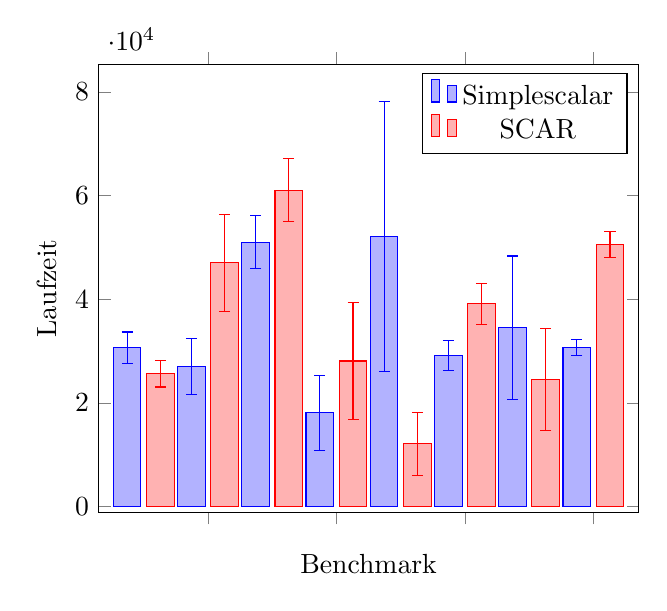
\begin{tikzpicture}
\begin{axis}[
    xlabel=Benchmark,
    ylabel=Laufzeit,
    ybar,
    xticklabels=data, 
    x tick label style={rotate=45, anchor=east, color=red}
]

\addplot+[error bars/.cd, y dir = both, y explicit relative] 
table [ x=Index, y=Wert, y error=Fehler] {
Index          Wert    Fehler  
1      	       30600 	0.1    
2	       27018 	0.2    
3	       51000 	0.1    
4	       18060 	0.4    
5	       52080    0.5    
6	       29100 	0.1    
7	       34512 	0.4    
8	       30600 	0.05  
};

\addplot+[error bars/.cd, y dir = both, y explicit relative] 
table [ x=Index, y=Wert, y error=Fehler] {
Index   Wert    Fehler
1	25600 	0.1
2	47010 	0.2
3	61000 	0.1
4	28060 	0.4
5	12080   0.5
6	39100 	0.1
7	24512 	0.4
8	50600 	0.05
};

\legend{Simplescalar, SCAR}
\end{axis}
\end{tikzpicture}






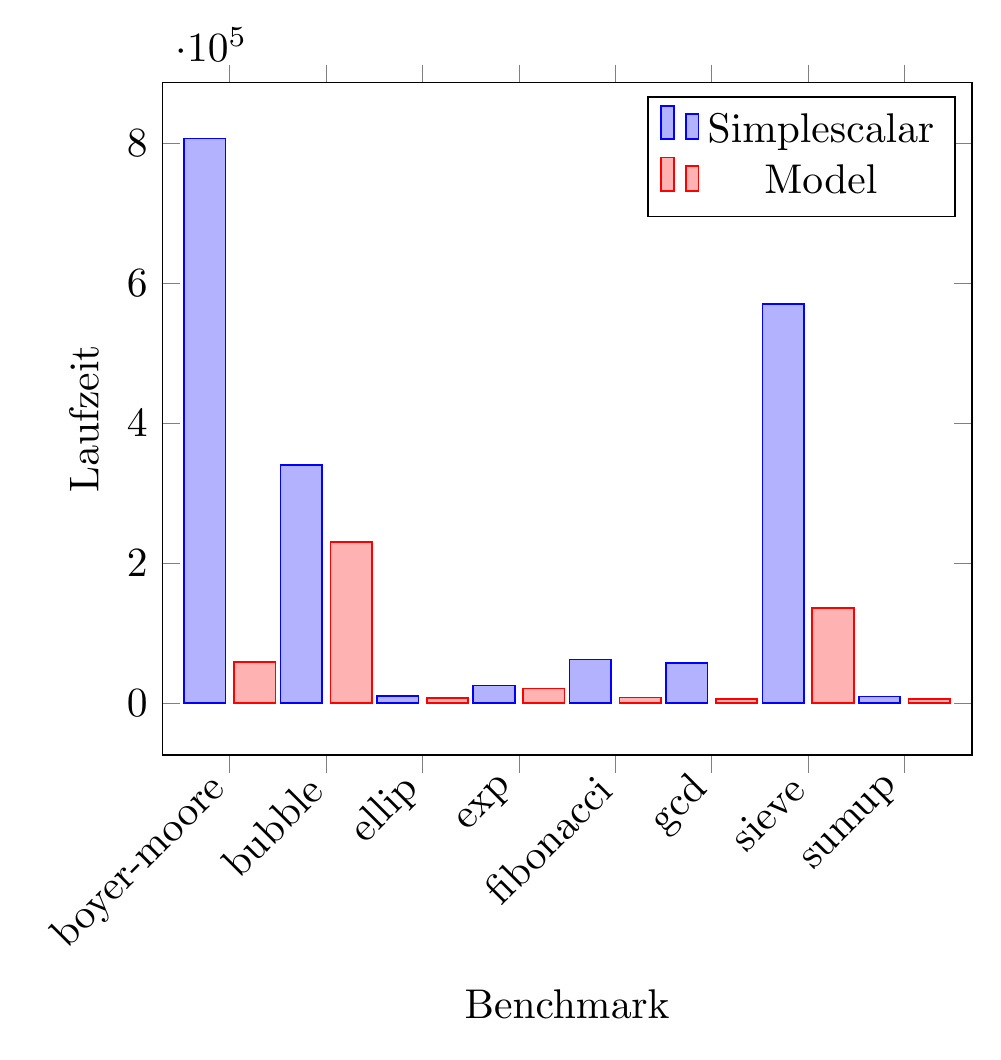
\begin{tikzpicture}[scale=1.5]
\begin{axis}[
    xlabel=Benchmark,
    ylabel=Laufzeit,
    ybar,
    xtick=data,
    xticklabels={boyer-moore, bubble, ellip, exp, fibonacci, gcd, sieve, sumup},
    x tick label style={rotate=45, anchor=east}
]
\addplot plot coordinates
  {
    (1, 806478)
    (2, 340228)
    (3, 10135)
    (4, 25099)
    (5, 62102)
    (6, 57111)
    (7, 570123)
    (8, 9592)
  };

\addplot plot coordinates
  {
    (1,59160)
    (2,230160)
    (3,7080)
    (4,21060)
    (5,8100)
    (6,6100)
    (7,136080)
    (8,6060)
  };
\legend{Simplescalar, Model}
\end{axis}
\end{tikzpicture}



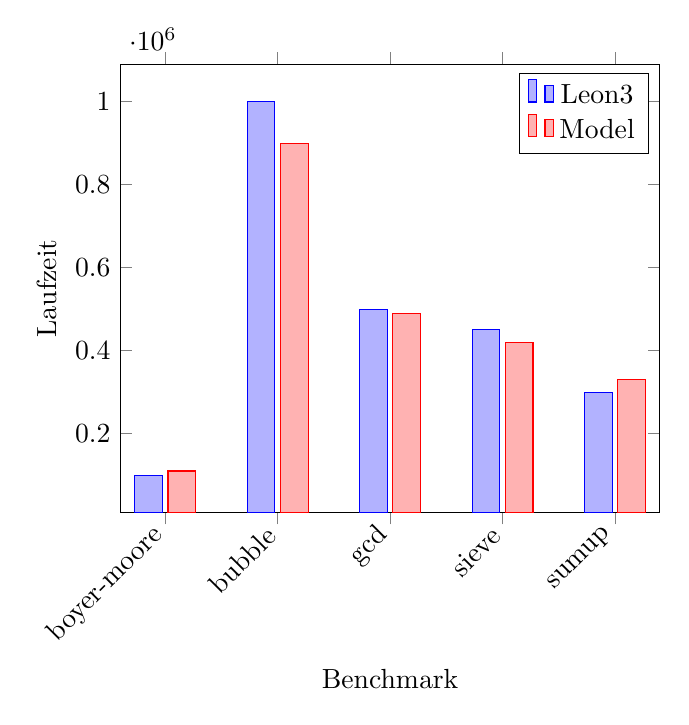
\begin{tikzpicture}
\begin{axis}[
    xlabel=Benchmark,
    ylabel=Laufzeit,
    ybar,
    xticklabels={,,boyer-moore, bubble, gcd, sieve, sumup},
    x tick label style={rotate=45, anchor=east}
]
\addplot plot coordinates
  {(1,100000) (2,1000000) (3,500000) (4,450000) (5,300000)};
\addplot plot coordinates
  {(1,110000) (2,900000) (3,490000) (4,420000) (5,330000)};
\legend{Leon3, Model}
\end{axis}
\end{tikzpicture}

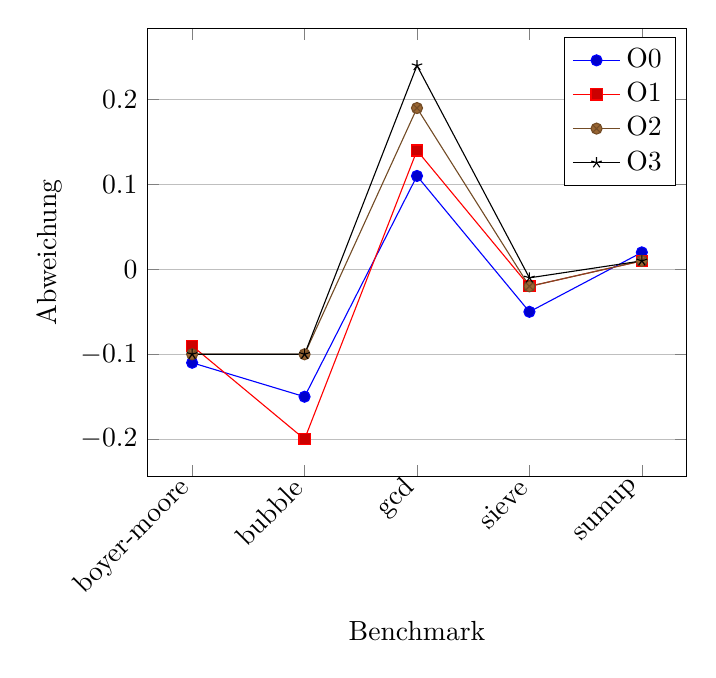
\begin{tikzpicture}
\begin{axis}[
    xlabel=Benchmark,
    ylabel=Abweichung,
    xticklabels={,,boyer-moore, bubble, gcd, sieve, sumup},
    x tick label style={rotate=45, anchor=east},
    ymajorgrids=true,
    yminorgrids=true
]
\addplot plot coordinates
  {(1,-0.11) (2,-0.15) (3,0.11) (4,-0.05) (5,0.02)};
\addplot plot coordinates
  {(1,-0.09) (2,-0.2) (3,0.14) (4,-0.02) (5,0.01)};
\addplot plot coordinates
  {(1,-0.1) (2,-0.1) (3,0.19) (4,-0.02) (5,0.01)};
\addplot plot coordinates
  {(1,-0.1) (2,-0.1) (3,0.24) (4,-0.01) (5,0.01)};

\legend{O0,O1,O2,O3}
\end{axis}
\end{tikzpicture}

% Pgfplots demo
% Author: Christian Feuersänger
% Source: Pgfplots manual:
% http://www.ctan.org/tex-archive/help/Catalogue/entries/pgfplots.html


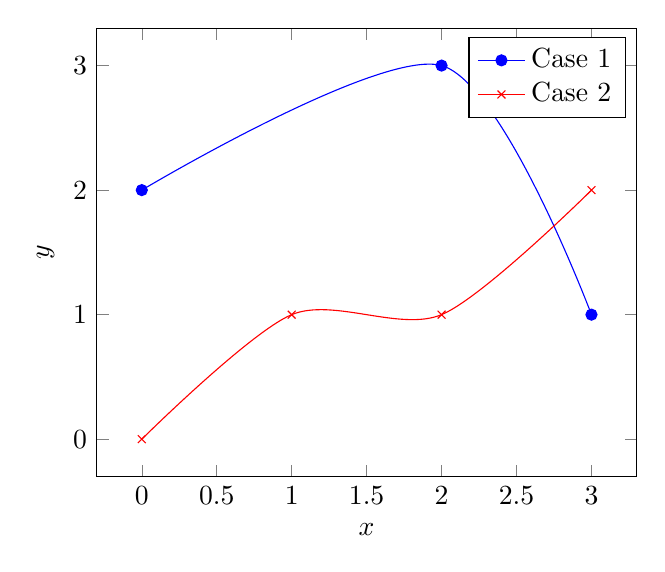
\begin{tikzpicture}
    \begin{axis}[
        xlabel=$x$,
        ylabel=$y$]
    \addplot[smooth,mark=*,blue] plot coordinates {
        (0,2)
        (2,3)
        (3,1)
    };
    \addlegendentry{Case 1}

    \addplot[smooth,color=red,mark=x]
        plot coordinates {
            (0,0)
            (1,1)
            (2,1)
            (3,2)
        };
    \addlegendentry{Case 2}
    \end{axis}
    \end{tikzpicture}


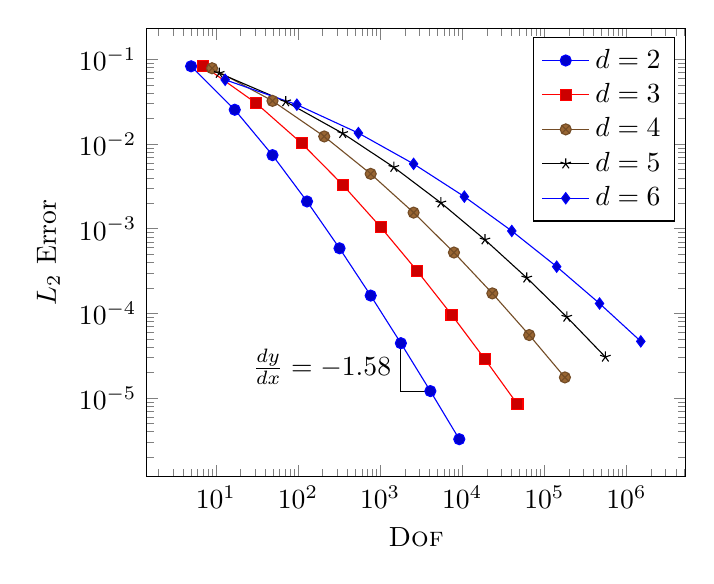
\begin{tikzpicture}
    \begin{loglogaxis}[
        xlabel=\textsc{Dof},
        ylabel=$L_2$ Error
    ]
    \axispath\draw
            (7.49165,-10.02171)
        |-  (8.31801,-11.32467)
        node[near start,left] {$\frac{dy}{dx} = -1.58$};
      \addplot plot coordinates {
        (5,     8.312e-02)
        (17,    2.547e-02)
        (49,    7.407e-03)
        (129,   2.102e-03)
        (321,   5.874e-04)
        (769,   1.623e-04)
        (1793,  4.442e-05)
        (4097,  1.207e-05)
        (9217,  3.261e-06)
    };

    \addplot plot coordinates {
        (7,     8.472e-02)
        (31,    3.044e-02)
        (111,   1.022e-02)
        (351,   3.303e-03)
        (1023,  1.039e-03)
        (2815,  3.196e-04)
        (7423,  9.658e-05)
        (18943, 2.873e-05)
        (47103, 8.437e-06)
    };

    \addplot plot coordinates {
        (9, 7.881e-02)
        (49,    3.243e-02)
        (209,   1.232e-02)
        (769,   4.454e-03)
        (2561,  1.551e-03)
        (7937,  5.236e-04)
        (23297, 1.723e-04)
        (65537, 5.545e-05)
        (178177,    1.751e-05)
    };

    \addplot plot coordinates {
        (11,    6.887e-02)
        (71,    3.177e-02)
        (351,   1.341e-02)
        (1471,  5.334e-03)
        (5503,  2.027e-03)
        (18943, 7.415e-04)
        (61183, 2.628e-04)
        (187903,    9.063e-05)
        (553983,    3.053e-05)
    };

    \addplot plot coordinates {
        (13,    5.755e-02)
        (97,    2.925e-02)
        (545,   1.351e-02)
        (2561,  5.842e-03)
        (10625, 2.397e-03)
        (40193, 9.414e-04)
        (141569,    3.564e-04)
        (471041,    1.308e-04)
        (1496065,   4.670e-05)
    };
    \legend{$d=2$\\$d=3$\\$d=4$\\$d=5$\\$d=6$\\}

    \end{loglogaxis}
\end{tikzpicture}

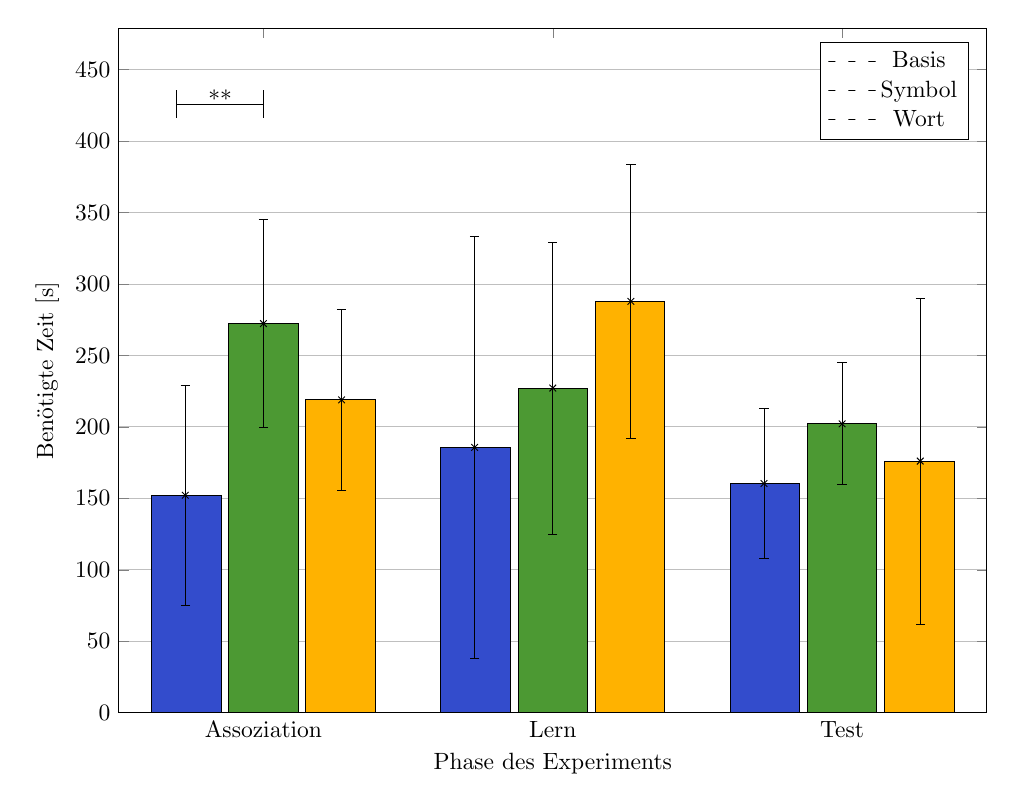
\begin{tikzpicture}[scale=0.85]

% defining custom colors
\definecolor{mycolor1}{rgb}{1,0.7,0}
\definecolor{mycolor2}{rgb}{0.3,0.6,0.2}
\definecolor{mycolor3}{rgb}{0.2,0.3,0.8}


\begin{axis}[
view={0}{90},
scale only axis,
width=5.10588in,
height=4.02706in,
xmin=0.5, xmax=3.5,
ymin=0, ymax=479.038,
xtick={1,2,3},
xticklabels={Assoziation,Lern,Test},
xlabel={Phase des Experiments},
ylabel={Benötigte Zeit [s]},
ymajorgrids]
\addplot[ybar,bar width=0.408471in, bar shift=-0.453856in,fill=mycolor3,draw=black] plot coordinates{ (1,152.189) (2,185.708) (3,160.405) };

\addplot[ybar,bar width=0.408471in, bar shift=0in,fill=mycolor2,draw=black] plot coordinates{ (1,272.288) (2,227.155) (3,202.183) };

\addplot[ybar,bar width=0.408471in, bar shift=0.453856in,fill=mycolor1,draw=black] plot coordinates{ (1,218.906) (2,287.852) (3,176.089) };

\addplot [
color=black,
only marks,
mark=x,
mark options={solid}
]
plot [error bars/.cd, y dir = both, y explicit]
coordinates{ (1,272.288) +- (0,72.84) (2,227.155) +- (0,102.09) (3,202.183) +- (0,42.583)
};
\addplot [
color=black,
only marks,
mark=x,
mark options={solid}
]
plot [error bars/.cd, y dir = both, y explicit]
coordinates{ (1.27,218.906) +- (0,63.028) (2.27,287.852) +- (0,96.089) (3.27,176.089) +- (0,113.98)
};
\addplot [
color=black,
only marks,
mark=x,
mark options={solid}
]
plot [error bars/.cd, y dir = both, y explicit]
coordinates{ (0.73,152.189) +- (0,76.984) (1.73,185.708) +- (0,147.64) (2.73,160.405) +- (0,52.605)
};

\addplot [
color=black,
solid
]
coordinates{ (0.7,425.918) (1,425.918)
};

\addplot [
color=black,
solid
]
coordinates{ (0.7,416.337) (0.7,435.499)
};

\addplot [
color=black,
solid
]
coordinates{ (1,416.337) (1,435.499)
};

\node at (axis cs:0.85, 430) {**};

\legend{Basis, Symbol, Wort}
\end{axis}
\end{tikzpicture}


\end{document}



